\section{Solving Adversarial Calibration}
\label{sec:calibration}
In this section,  we study the calibration of adversarial margin losses with regard to the adversarial $0/1$ loss. We first provide necessary and sufficient conditions under which margin losses are adversarially calibrated. We then show that a wide range of surrogate losses that are calibrated in the standard setting are not calibrated in the adversarial setting. Finally we propose a class of losses that are calibrated in the adversarial setting, namely the \emph{shifted odd losses}.

\subsection{Necessary and Sufficient Conditions for Calibration}

One of our main contributions is to find necessary and sufficient conditions for calibration in the adversarial setting. \textcolor{black}{In a brief, we identify that for studying calibration it is central to understand  the case where there might be indecision for classifiers (i.e. $\eta=1/2$)}. Indeed, in this case, either labelling positively or negatively the input $x$ would lead the same loss for $x$. Next result provides a necessary condition for calibration. 

\begin{thm}[Necessary condition for Calibration] 
\label{thm:calibration-nec}
Let $\phi$  be a continuous margin loss and $\varepsilon>0$. If $\phi$ is adversarially  calibrated at level $\varepsilon$, then $\phi$ is  calibrated in the standard classification setting and $0\not\in \argminB_{\alpha\in\bar{\RR}}
\frac12\phi(\alpha)+\frac12\phi(-\alpha)$. 
\end{thm}

While the condition of calibration in the standard classification setting seems natural, we need to understand why $0\not\in \argminB_{\alpha\in\bar{\RR}}
\frac12\phi(\alpha)+\frac12\phi(-\alpha)$. The intuition behind this result is that a sequence of functions simply converging towards $0$ in the ball of radius $\varepsilon$ around some $x$ can take positive and negative values thus leading to suboptimal $0/1$ adversarial risk. 

\begin{proof}

    Let us show that if $0\in\argminB_{\alpha\in\bar{\RR}} \phi(\alpha)+\phi(-\alpha)$ then $\phi$ is not calibrated for the adversarial problem. For that, let $x\in\mathcal{X}$ and we fix $\eta = \frac12$.  For $n\geq1$, we define $f_n(u) = \frac1n$ for $u\neq x$ and $-\frac{1}{n}$ for $u=x$.  Since $\lvert\mathcal{B}_\varepsilon(x)\rvert\geq 2$, we have
    \begin{align*}
         \mathcal{C}_{\phi_\varepsilon}(x,\frac12,f_n) = \max\left(\phi(\frac1n),\phi(-\frac1n)\right)\xrightarrow[n\to\infty]{} \phi(0) %= \inf_{\alpha\in\RR}\frac12\left(\phi(\alpha)+\phi(-\alpha)\right)
    \end{align*}
    As, $\phi(0) = \inf_{\alpha\in\bar{\RR}}\frac12\left(\phi(\alpha)+\phi(-\alpha)\right)$, the above means that $(f_n)_n$ is a minimizing sequence for $\alpha \mapsto \frac12 \left(\phi(\alpha)+\phi(-\alpha)\right)$. 
    Then thanks to Proposition~\ref{prop:calib-equality}, $(f_n)_n$ is also a minimizing sequence for $f \mapsto\mathcal{C}_{\phi_\varepsilon}(x,\frac12,f)$. However, for every integer $n$, we have $\mathcal{C}_{0/1,\varepsilon}(x,\frac12,f_n) =1\neq\frac12$. As  $\inf_{f\in\mathcal{F}(\XX)}\mathcal{C}_{\varepsilon}(x,\frac12,f)=\frac12$, $\phi$ is not calibrated with regard to the $0/1$ loss in the adversarial setting at level $\varepsilon$. We also immediately notice that if $\phi$ is  calibrated with regard to  $0/1$ loss in the adversarial setting at level $\varepsilon$ then $\phi$ is calibrated in the standard setting. 
    
    % Reciprocally, let us assume that  $\phi$ is calibrated in the standard setting and that if $0\not\in\argminB_\alpha \phi(\alpha)+\phi(-\alpha)$ then $\phi$ is  calibrated with to  $0/1$ loss in the adversarial setting at level $\varepsilon$.
    
\end{proof}



It turns out that, given an additional assumption, this condition is actually sufficient to ensure calibration.


\begin{thm}[Sufficient condition for Calibration] 
\label{thm:calibration-suf}
Let $\phi$  be a continuous margin loss and $\varepsilon>0$. If $\phi$ is decreasing and strictly decreasing in a neighbourhood of $0$ and calibrated in the standard setting and $0\not\in \argminB_{\alpha\in\bar{\RR}}
\frac12\phi(\alpha)+\frac12\phi(-\alpha)$, then $\phi$ is adversarially uniformly calibrated at level $\varepsilon$.
\end{thm}


\begin{proof}

    Let $\epsilon\in(0,\frac{1}{2})$. Thanks to Theorem~\ref{thm:cal-standard}, $\phi$ is uniformly calibrated in the standard setting, then there exists $\delta>0$, such that for all $x\in\mathcal{X}$, $\eta\in [0,1]$, $f\in \mathcal{F}(\XX)$:
    \begin{align*}
        \mathcal{C}_\phi(x,\eta,f) - \mathcal{C}_\phi^\star(x,\eta)\leq \delta \implies \mathcal{C}_{0/1}(x,\eta,f) - \mathcal{C}_{0/1}^\star(x,\eta)\leq \epsilon.
    \end{align*}
    
    % We first notice that when $\eta \neq \frac{1}{2}$, the adversarial calibration of $\phi$ ensures that for any minimizing sequence of the $\phi$ calibration function, the standard $0/1$ loss will be uniformly close to the optimal in a neighborhood of the point. This means that the classifier will remain of constant sign÷÷÷:÷÷÷ in that neighborhood, hence the adversarial calibration.
    
    \textbf{Case $\eta\neq \frac12$:} Let $x\in\mathcal{X}$ and $f\in \mathcal{F}(\XX)$ such that: 
    \begin{align*}
    \mathcal{C}_{\phi_\varepsilon}(x,\eta,f) - \mathcal{C}_{\phi_\varepsilon}^\star(x,\eta)
     = \sup_{u,v\in B_\varepsilon(x)}\eta\phi (f(u))+(1-\eta)\phi (-f(v))-\mathcal{C}_{\phi_\varepsilon}^\star(x,\eta)\leq \delta 
    \end{align*}
    We recall thanks to Proposition~\ref{prop:calib-equality} that for every $u,v\in\XX$,
\begin{align*}
    \mathcal{C}_{\phi_\varepsilon}^\star(u,\eta) =\mathcal{C}_\phi^\star(v,\eta)=\inf_{\alpha\in\RR}\eta \phi(\alpha)+(1-\eta)\phi(-\alpha)\quad.  
\end{align*}
 Then in particular, for all $x'\in B_\varepsilon(x)$, we have:
    \begin{align*}
        \mathcal{C}_{\phi}(x',\eta,f) - \mathcal{C}_{\phi}^\star(x',\eta)&\leq \sup_{u,v\in B_\varepsilon(x)}\eta\phi (f(u))+(1-\eta)\phi (-f(v))-\mathcal{C}_{\phi_\varepsilon}^\star(x,\eta)\\
        &\leq \delta\quad.
    \end{align*} 
    Then since $\phi$ is calibrated for standard classification, for all $x'\in B_\varepsilon(x)$, $\mathcal{C}(x',\eta,f) - \mathcal{C}^\star(x',\eta)\leq \epsilon$. Since,  $\epsilon<\frac{1}{2}$, we have $\mathcal{C}(x',\eta,f) = \mathcal{C}^\star(x',\eta)$ and then for all $x'\in B_\varepsilon(x)$, $f(x')< 0$  if $\eta<1/2$ or $f(x')\geq0$  if $\eta>1/2$. We then deduce that 
    
    \begin{align*}
       \mathcal{C}_{\varepsilon}(x,\eta,f)& = \eta \sup_{x'\in B_\varepsilon(x)} \mathbf{1}_{f(x')\leq 0 } +(1-\eta) \sup_{x'\in B_\varepsilon(x)} \mathbf{1}_{f(x')> 0 }\\
       & = \min(\eta,1-\eta)
        = \mathcal{C}_{\varepsilon}^\star(x,\eta)
    \end{align*}
    
    
    Then we deduce, $\mathcal{C}_{\varepsilon}(x,\eta,f) - \mathcal{C}_{\varepsilon}^\star(x,\eta)\leq \epsilon$.
    
    \medskip
    
    \textbf{Case $\eta=\frac12$:} This shows us that calibration problems will only arise when $\eta = \frac{1}{2}$, i.e. on points where the Bayes classifier is indecise. For this case, we will reason by contradiction: we can construct a sequence of points $\alpha_n$ and $\beta_n$, whose risks converge to the same optimal value, while one sequence remains close to some positive value, and the other to some negative value. Assume that for all $n$, there exist $f_n\in\mathcal{F}(\XX)$ and $x_n\in\XX$ such that 
    \begin{align*}
        \mathcal{C}_{\phi_\varepsilon}(x_n,\frac12,f_n) - \mathcal{C}_{\phi_\varepsilon}^\star(x_n,\frac12)\leq \frac1n 
    \end{align*}
    and there exists $u_n,v_n\in B_\varepsilon(x_n)$, such that 
    \begin{align*}
        f_n(u_n)f_n(v_n)\leq 0\quad 
    \end{align*} 
    Let us denote $\alpha_n = f_n(u_n)$ and $\beta_n = f_n(v_n)$. %Up to an extraction of a subsequence, we have $\alpha_n\xrightarrow[n\to\infty]{} \alpha\in \bar{\RR}$ and $\beta_n = f_n(u_n)\xrightarrow[n\to\infty]{} \beta\in \bar{\RR}$. 
    Moreover, we have thanks to Proposition~\ref{prop:calib-equality}:
    \begin{align*}
      0\leq \frac12 \phi(\alpha_n) +  \frac12 \phi(-\alpha_n)- \inf_{u\in\RR}\left[\frac12 \phi(u)+\frac12\phi(u)\right]&\leq \mathcal{C}_{\phi_\varepsilon}(x,\frac12,f_n) - \mathcal{C}_{\phi_\varepsilon}^\star(x,\frac12)\\
      &\leq \frac1n
    \end{align*}
    Then we deduce that $(\alpha_n)_n$ is a minimizing sequence for  $u\mapsto\frac12\phi(u)+\frac12\phi(-u)$ and similarly $(\beta_n)_n$ is also a minimizing sequence for  $u\mapsto\frac12\phi(u)+\frac12\phi(-u)$ . Now note that there always exist $\alpha, \beta\in \bar{\RR}$ such that, up to an extraction of a subsequence, we have $\alpha_n\xrightarrow[n\to\infty]{} \alpha$ and $\beta_n \xrightarrow[n\to\infty]{} \beta$. Furthermore by continuity of $\phi$ and since $0\not\in\argminB\phi(u)+\phi(-u)$, $\alpha\neq0$ and $\beta\neq 0$. Without loss of generality one can assume that $\alpha<0<\beta$, then for $n$ sufficiently large, $\alpha_n<0<\beta_n$. Moreover we have 
    \begin{align*}
         0&\leq\frac12\max\left(\phi(\alpha_n),\phi(\beta_n)\right)+\frac12\max\left(\phi(-\alpha_n),\phi(-\beta_n)\right)- \mathcal{C}^\star_{\phi_\varepsilon}(x,\frac12)\\
         &\leq \mathcal{C}_{\phi_\varepsilon}(x,\frac12,f_n) - \mathcal{C}_{\phi_\varepsilon}^\star(x,\frac12)\leq \frac1n
    \end{align*}
    so that we deduce:
    \begin{align}
    \label{eq:limitalphabeta}
     \frac12\max\left(\phi(\alpha_n),\phi(\beta_n)\right)+\frac12\max\left(\phi(-\alpha_n),\phi(-\beta_n)\right)\longrightarrow \inf_{u\in\RR}\left[\frac12 \phi(u)+\frac12\phi(u)\right]
    \end{align}
    
    Since, for $n$ sufficiently large, $\alpha_n<0<\beta_n$ and $\phi$ is decreasing  and strictly decreasing in a neighbourhood of $0$, we have that:
     $$\max\left(\phi(\alpha_n),\phi(\beta_n)\right) = \phi(\alpha_n)$$ and 
     $$\max\left(\phi(-\alpha_n),\phi(-\beta_n)\right) = \phi(-\beta_n)$$. Moreover, there exists $\lambda>0$ such that for $n$ sufficiently large $\phi(\alpha_n) - \phi(\beta_n)\geq \lambda$. Then for $n$ sufficiently large:
    \begin{align*}
        \frac12\max\left(\phi(\alpha_n),\phi(\beta_n)\right)&+\frac12\max\left(\phi(-\alpha_n),\phi(-\beta_n)\right)\\
         &= \frac{1}{2} \phi(\alpha_n) +\frac12 \phi(-\beta_n)\\
        &= \frac{1}{2} \left(\phi(\alpha_n)- \phi(\beta_n)\right)+\frac12 \phi(-\beta_n)+\frac{1}{2}+ \phi(\beta_n)\\
        &\geq \frac12\lambda +\inf_{u\in\RR}\left[\frac12 \phi(u)+\frac12\phi(u)\right]
    \end{align*}
    which leads to a contradiction with Equation~\ref{eq:limitalphabeta}. Then there exists a non zero integer $n_0$ such that for all $f\in\mathcal{F}(\XX)$, $x\in\XX$
    \begin{align*}
        \mathcal{C}_{\phi_\varepsilon}(x,\frac12,f) - \mathcal{C}_{\phi_\varepsilon}^\star(x,\frac12)\leq \frac{1}{n_0} \implies \forall u,v\in B_\varepsilon(x),~ f(u)\times f(v)> 0.
    \end{align*}
    
    The right-hand term is equivalent to: for all $u\in B_\varepsilon(x)$, $f(u)>0$ or for all $u\in B_\varepsilon(x)$, $f(u)<0$.  Then $\mathcal{C}_\varepsilon(x,\eta,f) =\frac12$ and then $\mathcal{C}_\varepsilon(x,\eta,f) = \mathcal{C}_\varepsilon^\star(x,\eta)$
    
    \medskip
    
    Putting all that together, for all $x\in\mathcal{X}$, $\eta\in [0,1]$, $f\in \mathcal{F}(\XX)$:
    \begin{align*}
        \mathcal{C}_{\phi_\varepsilon}(x,\eta,f) - \mathcal{C}_{\phi_\varepsilon}^\star(x,\eta)\leq \min(\delta,\frac{1}{n_0}) \implies \mathcal{C}_{\varepsilon}(x,\eta,f) - \mathcal{C}_{\varepsilon}^\star(x,\eta)\leq \epsilon.
    \end{align*}
    Then $\phi$ is adversarially uniformly calibrated at level $\varepsilon$
\end{proof}



% \begin{prv-sk*}
% The main idea of the proof is that the uniform calibration in the standard setting gives us some kind of continuity property on the adversarial calibration function, which guarantee that the optimal f will have the same sign for the surrogate and the $0/1$ as soon as $\eta \neq \frac{1}{2}$. Hence, calibration problems can only occur at places of uncertainty, i.e. $\eta = \frac{1}{2}$.

% When $\eta = \frac{1}{2}$, the $0/1$ loss still forces a decision. If the surrogate loss allows the "indecisive" optimum of 0, then we can construct a sequence of points that oscillate around 0, getting smaller but keeping opposite sign.
% \end{prv-sk*}


\begin{rmq}[Decreasing hypothesis] 




For the reciprocal, the additional assumption that $\phi$ is decreasing and strictly decreasing in a neighborhood of $0$ is not restrictive for usual losses. In Theorem~\ref{thm:cal-standard}, this assumption is stated as a necessary and sufficient condition for convex losses to be calibrated.
\end{rmq}





\subsection{Negative results}

Thanks to Theorem~\ref{thm:calibration-nec}, we can present two notable corollaries invalidating the use of two important classes of surrogate losses in the standard setting. The first class of losses are convex margin losses. These losses are maybe the most widely used in modern day machine learning as they comprise the logistic loss or the margin loss that are the building block of most classification algorithms. %\textcolor{blue}{[CITE Pytorch or else]}

\begin{coro} Let $\varepsilon>0$. Then no convex margin loss can be adversarially calibrated at level $\varepsilon$.
\end{coro} 
%$\phi$ a convex margin loss. Then, $\phi$ is not adversarially calibrated at level $\varepsilon$. 


A convex loss satisfies $\frac12\phi(\alpha)+\frac12\phi(-\alpha)\geq \phi(0)$, hence $0\in \argminB_{\alpha\in\RR}
\phi(\alpha)+\phi(-\alpha)$. From Theorem~\ref{thm:calibration-nec}, we deduce the result.   Then, $\phi$ is not adversarially calibrated at level $\varepsilon$. This result seems counter-intuitive and highlights the difficulty of optimizing and understanding the adversarial risk. Since  convex losses are not calibrated, one may hope to rely on  famous non-convex losses such as sigmoid and ramp losses. But, unfortunately, such losses are not either calibrated.




\begin{coro} Let $\varepsilon>0$. Let $\lambda\in \RR$ and \textcolor{black}{$\psi$} be a lower-bounded odd function such that for all $\alpha\in\RR$, $\psi>-\lambda$. We define $\psi$ as  $\phi(\alpha) = \lambda +\psi(\alpha)$. Then $\phi$ is not adversarially calibrated at level $\varepsilon$.
\end{coro}
Indeed, $\frac12{\phi}(\alpha)+\frac12{\phi}(-\alpha) =  \lambda$, so that $ \argminB_{\alpha\in\RR}
\frac12\phi(\alpha)+\frac12\phi(-\alpha) = \RR$. Thanks to Theorem~\ref{thm:calibration-nec}, $\phi$ is not adversarially calibrated at level $\varepsilon$.


\subsection{Positive results}

Theorem~\ref{thm:calibration-suf} also gives sufficient conditions for $\phi$ to be adversarially calibrated. Leveraging this result, we devise a class of margin losses that are indeed calibrated in the adversarial settings. We call this class \emph{shifted odd losses}, and we define it as follows.
\begin{definition}[Shifted odd losses]
\label{def:shifted}
We say that $\phi$ is a \emph{shifted odd margin loss} if there exists $\lambda\geq0$, $\tau>0$, and a continuous lower bounded strictly decreasing odd function \textcolor{black}{$\psi$} in a neighborhood of $0$ such that for all $\alpha\in\RR$, $\psi(\alpha)\geq -\lambda$ and $\phi(\alpha) = \lambda+\psi(\alpha-\tau)$. 
\end{definition}

The key difference between a standard odd margin loss and a shifted odd margin loss is the variations of the function $\alpha\mapsto\frac12\phi(\alpha)+\frac12\phi(-\alpha)$. 
The primary difference is that, in the standard case the optima of this function are located at $0$ while they are located in $-\infty$ and $+\infty$ in the adversarial setting. Let us give some examples of margin shifted odd losses below.

 
\begin{example*}[Shifted odd losses]
For every $\varepsilon>0$ and every $\tau>0$, the shifted logistic loss, defined as follows, is adversarially calibrated at level $\varepsilon$:
$\phi:\alpha\mapsto \left(1+\exp{\left(\alpha-\tau\right)}\right)^{-1}$
This loss is plotted on left in Figure~\ref{fig:cal}. We also plotted on right in Figure~\ref{fig:cal} $\alpha\mapsto\frac12\phi(\alpha)+\frac12\phi(-\alpha)$ to justify that $0\not\in\argminB_{\alpha\in\bar{\RR}}\frac12\phi(\alpha)+\frac12\phi(-\alpha)$. Also note that the shifted ramp loss also satisfies the same properties.
\end{example*}

A consequence of Theorem~\ref{thm:calibration-suf} is that shifted odd losses are adversarially calibrated, as demonstrated in Proposition~\ref{prop:calibrated-loss} stated below.

\begin{prop}
\label{prop:calibrated-loss}
Let $\phi$ be a shifted odd margin loss. For every $\varepsilon>0$, ${\phi}$ is adversarially calibrated at level $\varepsilon$.
\end{prop}


\begin{proof}
    Let $\lambda>0$, $\tau>0$ and $\phi$ be a strictly decreasing odd function such that $\Tilde{\phi}$ defined as  $\Tilde{\phi}(\alpha) = \lambda +\phi(\alpha-\tau)$ is non-negative. 
    
    \paragraph{Proving that $0\notin\argminB_{t\in\bar\RR}\frac12\Tilde{\phi}(t)+\frac12 \Tilde{\phi}(-t)$.}${\phi}$ is clearly strictly decreasing and non-negative then it admits a limit $l:=-\lim_{t\to+\infty}\Tilde{\phi}(t)\geq0$. Then we have:
    \begin{align*}
        \lim_{t\to+\infty}\Tilde{\phi}(t) = \lambda+l\quad\text{and}\quad\lim_{t\to-\infty}\Tilde{\phi}(t) = \lambda-l
    \end{align*}
    
    Consequently we have:
    \begin{align*}
        \lim_{t\to\infty}\frac12\Tilde{\phi}(t)+\frac12 \Tilde{\phi}(-t)= \lambda
    \end{align*}
    
    On the other side $\Tilde{\phi}(0)= \lambda + \phi(-\tau) >\lambda +\phi(0) =\lambda$ since $\tau>0$ and $\phi$ is strictly decreasing. Then $0\notin \argminB_{t\in\bar\RR}\frac12\Tilde{\phi}(t)+\frac12 \Tilde{\phi}(-t)$.
    
    % Let us even  show that $\argminB_t\frac12\Tilde{\phi}(t)+\frac12 \Tilde{\phi}(-t) = \{-\infty,+\infty\}$. We have for all $t$:
    % \begin{align*}
    %     \frac12\Tilde{\phi}(t)+\frac12\Tilde{\phi}(-t) &= \lambda +\frac12 \left(\phi(t-\tau)+\phi(-t-\tau)\right)\\
    %     & = \lambda +\frac12 \left(\phi(t-\tau)-\phi(t+\tau)\right)>\lambda
    % \end{align*}
    % since $t+\tau< t-\tau$ and $\phi$ is strictly decreasing. Hence by continuity of $\phi$ the optimum are attained when $t\to\infty$ or $t\to-\infty$. Then $\argminB_t\frac12\Tilde{\phi}(t)+\frac12 \Tilde{\phi}(-t) = \{-\infty,+\infty\}$.
    
    \paragraph{Proving that $\Tilde{\phi}$ is calibrated for standard classification.} Let $\epsilon>0$, $\eta\in[0,1]$, $x\in\mathcal{X}$. If $\eta=\frac12$, then for all $f\in\mathcal{F}(\XX)$, $\mathcal{C}(x,\frac12,f)= \mathcal{C}^\star(x,\frac12)=\frac12$. Let us now assume that $\eta\neq\frac12$, we have for all $f\in\mathcal{F}(\XX)$:
    
    \begin{align*}
         \mathcal{C}_{\Tilde{\phi}}(x,\eta,f) &= \lambda + \eta\phi(f(x)-\tau) + (1-\eta)\phi(-f(x)-\tau)\\
         &= \lambda + (\eta-\frac12)\left(\phi(f(x)-\tau)-\phi(-f(x)-\tau)\right)\\
         &+\frac12 \left(\phi(f(x)-\tau)+\phi(-f(x)-\tau)\right)
    \end{align*}
    
    
    Let us  show that $\argminB_{t\in\bar{\RR}}\frac12\Tilde{\phi}(t)+\frac12 \Tilde{\phi}(-t) = \{-\infty,+\infty\}$. We have for all $t$:
    \begin{align*}
        \frac12\Tilde{\phi}(t)+\frac12\Tilde{\phi}(-t) &= \lambda +\frac12 \left(\phi(t-\tau)+\phi(-t-\tau)\right)\\
        & = \lambda +\frac12 \left(\phi(t-\tau)-\phi(t+\tau)\right)>\lambda
    \end{align*}
    since $t-\tau< t+\tau$ and $\phi$ is strictly decreasing. Hence by continuity of $\phi$ the optimum are attained when $t\to\infty$ or $t\to-\infty$. Then $\argminB_{t\in\bar{\RR}}\frac12\Tilde{\phi}(t)+\frac12 \Tilde{\phi}(-t) = \{-\infty,+\infty\}$.
    
    Without loss of generality, let $\eta>1/2$, then
    \begin{align*}
        t\mapsto  (\eta-\frac12)\left(\phi(t-\tau)-\phi(-t-\tau)\right)
    \end{align*}
    is strictly decreasing and 
        $\argminB_{t\in\bar{\RR}}\frac12 \left(\phi(t-\tau)+\phi(-t-\tau)\right) = \{-\infty,+\infty\}$, then we have 
    \begin{align*}
        \argminB_{t\in\bar{\RR}} \lambda + (\eta-\frac12)\left(t-\tau)-\phi(-t-\tau)\right)+\frac12 \left(\phi(t-\tau)+\phi(-t-\tau)\right) = \{+\infty\}\quad.
    \end{align*}
     By continuity of $\phi$, we deduce that for $\delta>0$ sufficiently small:
    \begin{align*}
        \mathcal{C}_{\Tilde{\phi}}(x,\eta,f)-&\mathcal{C}^\star_{\Tilde{\phi}}(x,\eta)\leq\delta\implies f(x)>0
    \end{align*}
    
    The same reasoning holds for $\eta<\frac12$. Then we deduce that $\Tilde{\phi}$ is calibrated for standard classification.
    
    \medskip
    
    Finally, we obtain that  $\Tilde{\phi}$ is calibrated for adversarial classification for every $\varepsilon>0$.
\end{proof}




    
    



\begin{figure}
    \centering
    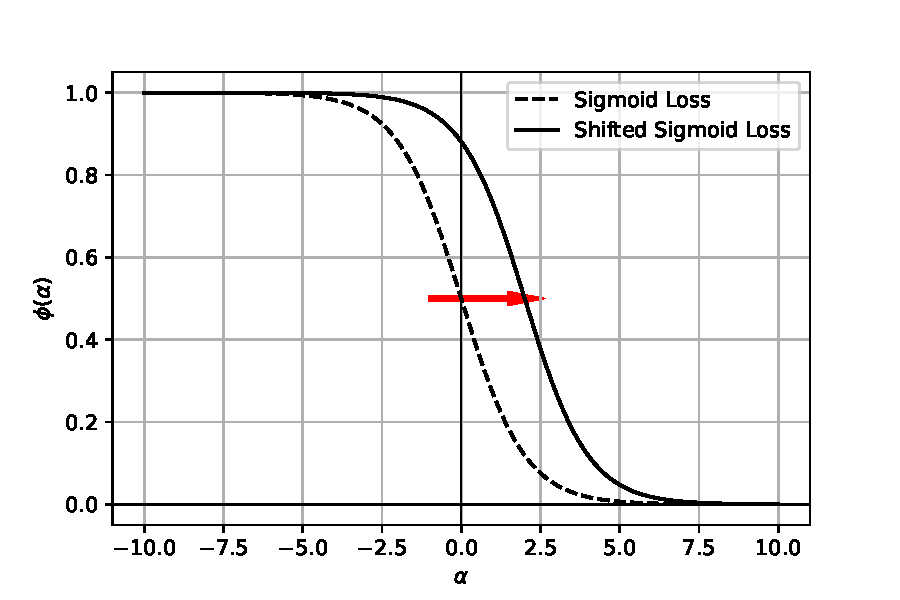
\includegraphics[width = 0.45\textwidth]{sections/3_calibration/images/calibrated_loss.pdf}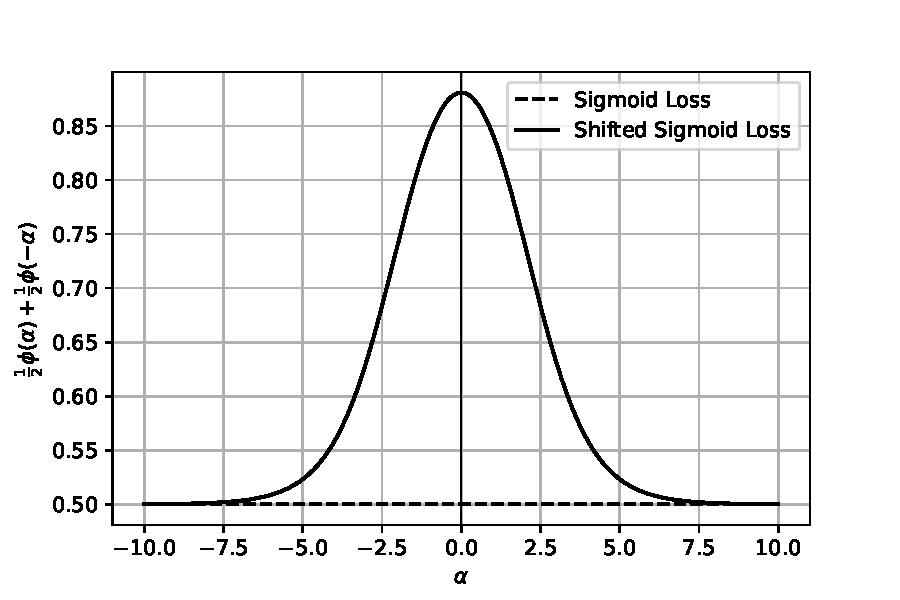
\includegraphics[width = 0.45\textwidth]{sections/3_calibration/images/calibrated_loss_ass.pdf}
    \caption{Illustration of the a calibrated loss in the adversarial setting. The sigmoid loss satisfy the hypothesis for $\psi$. Its shifted version is then calibrated for adversarial classification.}
    \label{fig:cal}
\end{figure}






\subsection{About $\mathcal{H}$-calibration}
\label{sec:hcal}
Our results naturally extend to $\mathcal{H}$-calibration. With mild assumptions on $\mathcal{H}$, it is possible to recover all the results made on calibration on $\mathcal{F}(\XX)$. First, it is worth noting that, if $\mathcal{H}$ contains all constant functions, then most results about calibration in the adversarial setting extend. Proposition~\ref{prop:calib-equality}  naturally extends to $\mathcal{H}$-calibration as long as $\mathcal{H}$ contains all constant functions. 


\begin{prop*}
\label{prop:hcalequality}
Let $\mathcal{H}\subset \mathcal{F}(\mathcal{X})$. Let us assume that $\mathcal{H}$ contains all constant functions. Let $\varepsilon>0$ and $\phi$ be a continuous classification margin loss.  For all $x\in\mathcal{X}$ and $\eta\in[0,1]$, we have
\begin{align*}
    \mathcal{C}^\star_{\phi_\varepsilon,\mathcal{H}}(x,\eta)=\mathcal{C}^\star_{\phi,\mathcal{H}}(x,\eta) =\inf_{\alpha\in\RR}\eta \phi(\alpha)+(1-\eta)\phi(-\alpha)= \mathcal{C}^\star_{\phi_\varepsilon}(x,\eta)=\mathcal{C}^\star_{\phi}(x,\eta)\quad.
\end{align*}
The last equality also holds for the adversarial $0/1$ loss.
\end{prop*}
The proof is exactly the same as for Proposition~\ref{prop:calib-equality} since we used a constant function to prove the equality. Under the same assumptions, the notion of $\mathcal{H}$-calibration and uniform $\mathcal{H}$-calibration are equivalent in the standard setting.




\begin{prop*}
Let $\mathcal{H}\subset \mathcal{F}(\mathcal{X})$. Let us assume that $\mathcal{H}$ contains all constant functions. Let $\phi$ be a continuous classification margin loss.  $\phi$ is uniformly $\mathcal{H}$-calibrated for standard classification if and only if  $\phi$ is uniformly calibrated for standard classification. It also holds for non-uniform calibration.
\end{prop*}
\begin{proof}
Let us assume that $\phi$ is a continuous classification margin loss and that $\phi$ is uniformly calibrated. Let $\epsilon>0$. There exists $\delta>0$ such that, for all $\eta\in[0,1]$, $x\in\mathcal{X}$ and $f\in\mathcal{F}(\XX)$:
\begin{align*}
    \mathcal{C}_{\phi}(x,\eta,f)- \mathcal{C}^\star_{\phi}(x,\eta)\leq\delta\implies\mathcal{C}(x,\eta,f)- \mathcal{C}^\star(x,\eta)\leq \epsilon\quad.
\end{align*}

Let $\eta\in[0,1]$, $x\in\mathcal{X}$ and $f\in\mathcal{H}$ such that $ \mathcal{C}_{\phi}(x,\eta,f)- \mathcal{C}^\star_{\phi,\mathcal{H}}(x,\eta)\leq\delta$. Thanks to Proposition~\ref{prop:hcalequality}, $\mathcal{C}^\star_{\phi,\mathcal{H}}(x,\eta)=\mathcal{C}^\star_{\phi}(x,\eta)$, and $f\in\mathcal{F}(\XX)$, then $\mathcal{C}_{\phi}(x,\eta,f)- \mathcal{C}^\star_{\phi}(x,\eta)\leq\delta$ and  then:
\begin{align*}
    \mathcal{C}(x,\eta,f)- \mathcal{C}^\star_{\mathcal{H}}(x,\eta) =  \mathcal{C}(x,\eta,f)- \mathcal{C}^\star(x,\eta) \leq\epsilon
\end{align*}
Then $\phi$ is uniformly $\mathcal{H}$-calibrated in standard classification.

Reciprocally, let us assume that $\phi$ is a continuous classification margin loss and that $\phi$ is uniformly $\mathcal{H}$-calibrated. Let $\epsilon>0$. There exists $\delta>0$ such that, for all $\eta\in[0,1]$, $x\in\mathcal{X}$ and $f\in\mathcal{H}$:
\begin{align*}
    \mathcal{C}_{\phi}(x,\eta,f)- \mathcal{C}^\star_{\phi,\mathcal{H}}(x,\eta)\leq\delta\implies\mathcal{C}(x,\eta,f)- \mathcal{C}^\star_\mathcal{H}(x,\eta)\leq \epsilon\quad.
\end{align*}


Let $\eta\in[0,1]$, $x\in\mathcal{X}$ and $f\in\mathcal{H}$ such that $ \mathcal{C}_{\phi}(x,\eta,f)- \mathcal{C}^\star_{\phi,\mathcal{H}}(x,\eta)\leq\delta$.  $\mathcal{C}_{\phi}(x,\eta,f) = \eta\phi(f(x))+(1-\eta)\phi(-f(x))$. Let $\Tilde{f}:u\mapsto f(x)$ for all $u\in\mathcal{X}$, then $\Tilde{f}\in\mathcal{H}$ since $\Tilde{f}$ is constant, $\mathcal{C}_{\phi}(x,\eta,f) = \mathcal{C}_{\phi}(x,\eta,\Tilde{f})$ and $\mathcal{C}(x,\eta,f) = \mathcal{C}(x,\eta,\Tilde{f})$. Thanks to the previous proposition, $\mathcal{C}^\star_{\phi,\mathcal{H}}(x,\eta)=\mathcal{C}^\star_{\phi}(x,\eta)$. Then: $ \mathcal{C}_{\phi}(x,\eta,\Tilde{f})-\mathcal{C}^\star_{\phi,\mathcal{H}}(x,\eta)\leq \delta$ and then:
\begin{align*}
    \mathcal{C}(x,\eta,f)-\mathcal{C}^\star_{\phi,\mathcal{H}}(x,\eta) =  \mathcal{C}(x,\eta,\Tilde{f})-\mathcal{C}^\star_{\phi}(x,\eta) \leq \epsilon
\end{align*}
Then $\phi$ is uniformly calibrated in standard classification.
\end{proof}

We can now obtain the necessary and sufficient conditions as follows. They are really similar to the adversarial calibration ones. 



\begin{prop*}[Necessary conditions for $\mathcal{H}$-Calibration of adversarial losses] 
Let $\varepsilon>0$. Let $\mathcal{H}\subset \mathcal{F}(\mathcal{X})$. Let us assume that $\mathcal{H}$ contains all constant functions and that there exists $x\in\XX$ and $(f_n)_n\in\mathcal{H}^\mathbb{N}$ such that $f_n(u)\to 0$ for all $ u\in B_\varepsilon(x)$ and for all $n\in\mathbb{N}$, $\sup_{u\in B_\varepsilon(x)} f_n(u)>0$ and  $\inf_{u\in B_\varepsilon(x)} f_n(u)<0$ 
Let $\phi$  be a continuous margin loss .  If $\phi$ is adversarially uniformly $\mathcal{H}$-calibrated at level $\varepsilon$, then $\phi$ is uniformly calibrated in the standard classification setting and $0\not\in \argminB_{\alpha\in\bar{\RR}}
\frac12\phi(\alpha)+\frac12\phi(-\alpha)$. 

\end{prop*}

\begin{prop*}[Sufficient conditions for $\mathcal{H}$-Calibration of adversarial losses]
Let $\mathcal{H}\subset \mathcal{F}(\mathcal{X})$. Let us assume that $\mathcal{H}$ contains all constant functions.
Let $\phi$  be a continuous strictly decreasing margin loss and $\varepsilon>0$. If $\phi$ is calibrated in the standard classification setting and $0\not\in \argminB_{\alpha\in\bar{\RR}}
\frac12\phi(\alpha)+\frac12\phi(-\alpha)$, then $\phi$ is adversarially uniformly $\mathcal{H}$-calibrated at level $\varepsilon$.x


\end{prop*}

The proofs are the same as for the adversarial calibration setting. Note however that the assumptions on $\mathcal{H}$ are very weak: for instance, the set of linear classifiers 
\begin{align*}
    \mathcal{H}=\left\{x\mapsto \langle w,x\rangle +b\mid w\in\RR^d,b\in \RR \right\}
\end{align*}
satisfies the existence of $x\in\XX$ and $(f_n)_n\in\mathcal{H}^\mathbb{N}$ such that $f_n(u)\to 0$ for all $ u\in B_\varepsilon(x)$ and for all $n\in\mathbb{N}$, $\sup_{u\in B_\varepsilon(x)} f_n(u)>0$ and  $\inf_{u\in B_\varepsilon(x)} f_n(u)<0$. 